% !TEX program = xelatex
% 光遗传学与视觉功能恢复 · 上海等级考风格综合题（22 分 / 8 小问）
% 编译：xelatex -interaction=nonstopmode -halt-on-error 本文件（跑两遍）
\documentclass[UTF8,a4paper,11pt]{ctexart}

\usepackage{geometry}
\geometry{left=1.9cm,right=1.9cm,top=2.3cm,bottom=2.3cm}
\usepackage{graphicx}
\usepackage{amsmath,amssymb}
\usepackage{booktabs}
\usepackage{longtable}
\usepackage{array}
\usepackage{enumitem}
\usepackage{xcolor}
\usepackage{caption}
\usepackage{float}
\usepackage{titlesec}
\usepackage{fancyhdr}
\usepackage[hidelinks]{hyperref}

\graphicspath{{../命题图/}{../../Resources/Downloads/原图-光遗传学视觉恢复/}}

\definecolor{deepblue}{HTML}{1F4E79}
\definecolor{deepred}{HTML}{C00000}
\definecolor{deepgreen}{HTML}{2E7D32}
\definecolor{greybg}{HTML}{F2F2F2}

\captionsetup{font=small,labelfont=bf}
\titleformat{\section}{\Large\bfseries\color{deepblue}}{\thesection}{0.6em}{}
\titleformat{\subsection}{\large\bfseries\color{deepblue}}{\thesubsection}{0.6em}{}
\pagestyle{fancy}
\fancyhf{}
\fancyhead[L]{\small 光遗传学与视觉功能恢复 · 上海等级考风格综合题}
\fancyhead[R]{\small\thepage}

\newcommand{\pt}[1]{\textbf{（#1分）}}
\newcommand{\tg}[1]{{\small\color{deepgreen}［#1］}}
\newcommand{\key}[1]{\textbf{\color{deepred}#1}}
\newcommand{\tian}[1]{\underline{\hspace{#1}}}
\newcommand{\choice}[1]{\par\smallskip\noindent #1\par}

\title{\bfseries 光遗传学与视觉功能恢复\\[5pt]\large 上海高中生物学等级考风格综合题\\[4pt]
\normalsize 22 分 / 8 小问 / 3 图表（含命题审查报告）}
\author{}\date{2026-10-06}

\begin{document}
\maketitle
\thispagestyle{fancy}

\begin{center}
\fbox{\parbox{0.95\textwidth}{\small
\textbf{阅读提示}：本卷所有科研事实均取自三篇开放获取论文（Pan et al. 2014；Lu et al. 2016；Lu et al. 2018）；
表中数值凡标"\textbf{命题简化}"者，其\emph{量级与具体数值为命题需要而设定}，但\emph{变化趋势}依据原论文结果改写，不改变科学结论。
}}
\end{center}

\section*{A\quad 命题逻辑图}
\addcontentsline{toc}{section}{A\quad 命题逻辑图}

\begin{center}
\small
\fbox{视网膜感光细胞退化}\ $\rightarrow$\ \fbox{视觉信号形成受阻}\ $\rightarrow$\ \fbox{ChR2 使残存细胞获得光响应}\\[4pt]
$\downarrow$\hfill（B 段：基础）\hfill（C 段：机制与突变体）\hfill\\[2pt]
\fbox{AAV 递送 + 特异性启动子}\ $\rightarrow$\ \fbox{比较 ChR2 变体的功能}\ $\rightarrow$\ \fbox{OMR 行为学评价}\ $\rightarrow$\ \fbox{综合优化}\\[4pt]
（E 段：基因工程）\hfill（D 段：多指标权衡）\hfill（F 段：实验设计）\hfill（G 段：评价）
\end{center}

\noindent\textbf{推理链}：认识现象（Q1）→ 提取证据（Q2、Q4）→ 比较与判断（Q4、Q6）→ 机制解释（Q3、Q5）→ 实验验证（Q7）→ 综合评价（Q8）。

\section{B\quad 完整题目（最终版）}
\addcontentsline{toc}{section}{B\quad 完整题目（最终版）}

\subsection*{材料}

视网膜色素变性（RP）是一类由基因突变引起的遗传性眼病。患者视网膜中的\textbf{感光细胞}逐渐死亡，而内层的\textbf{双极细胞}与\textbf{神经节细胞}大多仍然存活（图1）。感光细胞一旦大量死亡，视觉信号在视网膜的\textbf{第一站}就无法形成，患者因而逐渐失明。

研究者尝试用\textbf{光遗传学}方法恢复视觉：把一种来自单细胞藻类的光敏蛋白基因（ChR2 基因）经改造后，用腺相关病毒（AAV）作载体送入视网膜，使残存的视网膜细胞"感光化"。为让目的基因尽可能只进入并表达在\textbf{双极细胞}中，研究者比较了两套调控方案；为提高细胞在弱光下的反应能力，他们还构建了 ChR2 的多种\textbf{突变体}（表1）。最后，研究者用\textbf{视动反应（OMR）}——小鼠头部随视野中移动条纹产生的跟随运动——来评价视觉功能是否真正恢复（图2）。此外，为确认目的基因是否"送对了地方"，研究者把 ChR2 与红色荧光蛋白 mCherry 融合，并用能特异标记\textbf{视杆双极细胞}的 PKC 抗体作对照（图3）。

\begin{figure}[H]
\centering
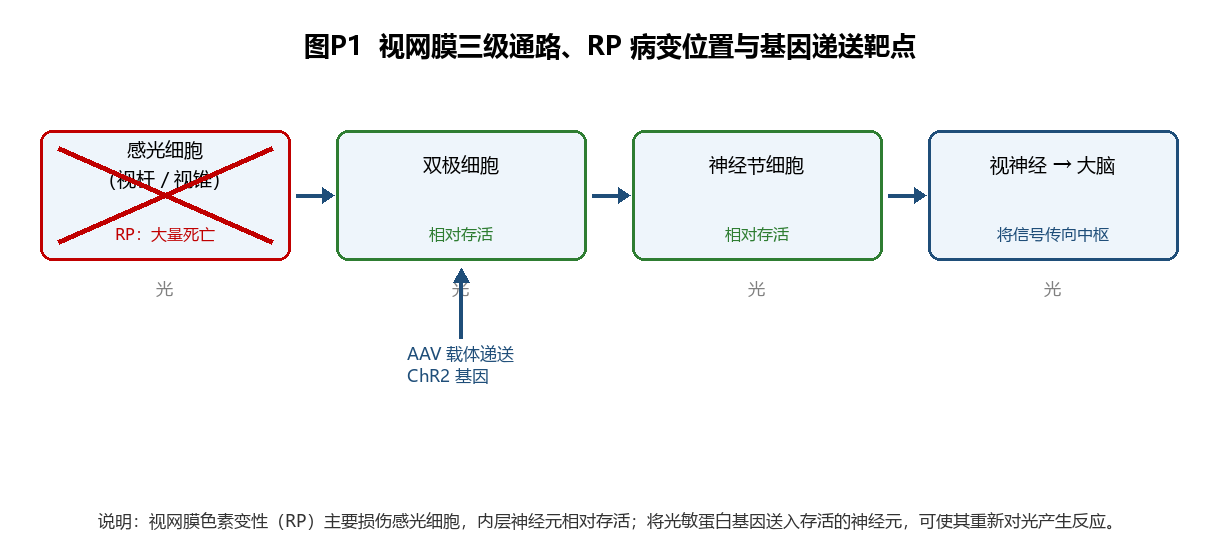
\includegraphics[width=0.95\textwidth]{P1_视网膜三级通路与病变.png}
\caption{图1\quad 视网膜三级细胞通路、RP 主要受损环节（\%）与治疗靶点（简化示意图）}
\end{figure}

\begin{table}[H]
\centering
\small
\caption*{\textbf{表1}\quad ChR2 及其突变体的功能比较（\key{命题简化}数据，相对值）}
\begin{tabular}{@{}lccc@{}}
\toprule
\textbf{变体} & \textbf{弱光下相对光电流} & \textbf{通道关闭（失活）时间} & \textbf{对快速变化光信号的跟随能力} \\
\midrule
wt-ChR2 & 1.0 & 最短 & 最强 \\
ChR2-L132C & 2.4 & 较长 & 较弱 \\
ChR2-L132C/T159C & 3.1 & 长 & 弱 \\
ChR2-L132C/T159S & 4.0 & 最长 & 最弱 \\
\bottomrule
\end{tabular}

\smallskip
\parbox{0.93\textwidth}{\footnotesize 注：光电流越大，说明细胞在\emph{越弱的光}下即可被激活（光敏性越高）；通道关闭越慢，细胞\emph{恢复}到静息状态所需时间越长，对随时间快速变化的光信号（如运动物体的位置变化）的跟随能力越弱。趋势依据 Pan et al., 2014 改写，数值为命题简化。}
\end{table}

\begin{table}[H]
\centering
\small
\caption*{\textbf{表2}\quad 两套调控方案的表达效果比较（\key{命题简化}数据，相对水平）}
\begin{tabular}{@{}lccc@{}}
\toprule
\textbf{方案} & \textbf{表达目的基因的视网膜细胞数量} & \textbf{其中双极细胞所占比例} & \textbf{单个细胞荧光强度} \\
\midrule
甲：200 bp 增强子 + SV40 启动子 & 较少（基准） & 中等 & 中等 \\
乙：内源 mGluR6 启动子 + 内含子增强子 & 明显增多 & 高 & 较高 \\
\bottomrule
\end{tabular}

\smallskip
\parbox{0.93\textwidth}{\footnotesize 注：两套方案均含有相同的 ChR2 基因编码序列与病毒衣壳，区别只在于与目的基因连接的\textbf{调控元件}不同；趋势依据 Lu et al., 2016 结果改写，数值为命题简化。}
\end{table}

\begin{figure}[H]
\centering
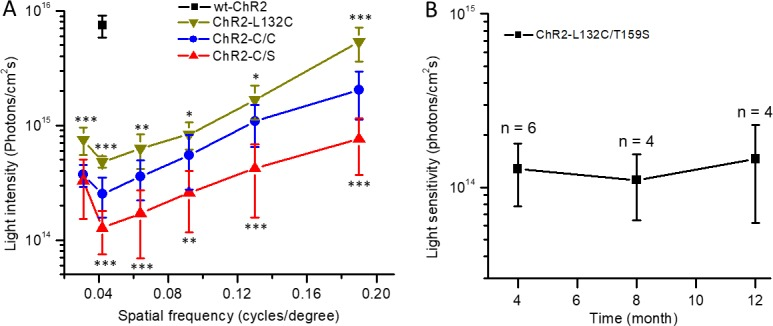
\includegraphics[width=1.0\textwidth]{Lu2018-Fig04.jpg}
\caption{图2\quad 论文原图（Lu et al., \textit{IOVS}, 2018, Fig.~4）：三种 ChR2 变体小鼠的视动反应（OMR）阈值光强与空间频率（条纹密集程度）的关系}
\end{figure}

\begin{figure}[H]
\centering
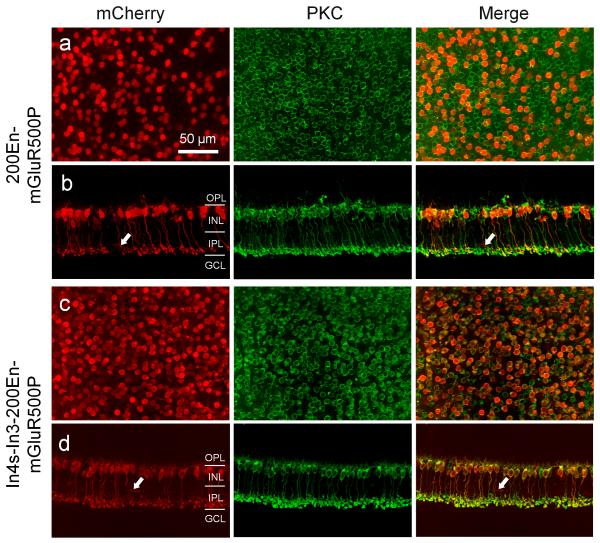
\includegraphics[width=1.0\textwidth]{Lu2016-Fig04.jpg}
\caption{图3\quad 论文原图（Lu et al., \textit{Gene Therapy}, 2016, Fig.~4）：mCherry（红）与视杆双极细胞标记 PKC 的共标结果}
\end{figure}

\subsection*{小问（共 22 分）}

\begin{enumerate}[leftmargin=2.1em,itemsep=5pt]
\item \tg{单选} \pt{2} 在视网膜中，直接把光信号转变为电信号的细胞是（\quad）\\
\choice{A. 感光细胞 \quad B. 双极细胞 \quad C. 神经节细胞 \quad D. 水平细胞}

\item \tg{多选} \pt{2} 结合材料与所学知识，下列关于 RP 与光遗传学治疗的叙述，合理的有（\quad）（错选得 0 分）\\
\choice{A. RP 患者感光细胞大量死亡后，双极细胞与神经节细胞通常仍能存活\\
B. 把 ChR2 基因导入双极细胞后，双极细胞在蓝光照射下也能产生电位变化\\
C. 该治疗直接修复了患者致病的基因，因而能从根本上治愈 RP\\
D. 治疗后，视觉信号仍需经神经节细胞上传至大脑皮层视觉中枢，才能形成视觉}

\item \tg{编号排序} \pt{2} 用编号和箭头（→）表示"导入 ChR2 基因后，双极细胞对蓝光产生反应"的过程顺序：\\
\choice{① ChR2 基因转录、翻译出 ChR2 蛋白 \quad ② 重组载体进入双极细胞\\
③ 蓝光照射下通道开放、阳离子内流 \quad ④ ChR2 定位到细胞膜上 \quad ⑤ 膜电位改变，产生电信号\\
答：\tian{7.2cm}}

\item \tg{表格填空} \pt{3} 据表1 完成下列填空：
\begin{enumerate}[label=(\arabic*),leftmargin=1.4em,itemsep=2pt]
\item 四种变体按"弱光下相对光电流"由大到小排序：\tian{6.6cm}
\item 若要让细胞尽可能准确地跟随随时间快速变化的光信号，应优先选择\tian{2.4cm}（填变体名称）
\end{enumerate}

\item \tg{简答} \pt{3} 有人认为"临床上应直接选择光敏性最高的变体"。请结合表1 评价这一观点，并说明理由。

\item \tg{编号选填 + 简答} \pt{3}
\begin{enumerate}[label=(\arabic*),leftmargin=1.4em,itemsep=2pt]
\item 据表2，若既要提高转导效率、又要使表达尽量集中在双极细胞中，应选择的方案是\tian{0.8cm}（填"甲"或"乙"）
\item 结合图3，说明研究者判断"目的基因是否主要在目标细胞中表达"的思路。
\end{enumerate}

\item \tg{实验方案完善} \pt{4} 研究者用失明小鼠评价治疗效果（结果见图2）。
\begin{enumerate}[label=(\arabic*),leftmargin=1.4em,itemsep=2pt]
\item \pt{2} 写出该实验的\textbf{自变量}与\textbf{因变量}，并说明需要控制相同的两个条件。
\item \pt{2} 有同学认为"只要检测视网膜中 ChR2 的表达量，就能判断视觉功能恢复的程度"。结合图2 评价这一说法。
\end{enumerate}

\item \tg{综合优化} \pt{3}
\begin{enumerate}[label=(\arabic*),leftmargin=1.4em,itemsep=2pt]
\item \pt{1} 现有两个改进方向：\textbf{①} 继续筛选光敏性更高、但时间响应更慢的变体；\textbf{②} 优化调控元件使表达更集中，同时筛选时间响应更好的变体。请选择更合理的方向并说明理由。
\item \pt{2} 结合上述材料，提出一条进一步优化的方向（可以是治疗方案的任何环节），并说明理由。
\end{enumerate}
\end{enumerate}

\section{C\quad 标准答案}
\addcontentsline{toc}{section}{C\quad 标准答案}

\begin{enumerate}[leftmargin=2.1em,itemsep=4pt]
\item \textbf{A（感光细胞）}。
\item \textbf{ABD}。C 错：光遗传学并没有修复致病基因，而是让残存的细胞"获得"光响应能力，属于"绕过受损环节"的功能补偿，并非根治。
\item \textbf{②→①→④→③→⑤}。
\item （1）\textbf{ChR2-L132C/T159S → ChR2-L132C/T159C → ChR2-L132C → wt-ChR2}；（2）\textbf{wt-ChR2}。
\item 该观点\textbf{不全面}。理由：① 表1 显示"光敏性（弱光下光电流大小）"与"时间响应（通道关闭快慢、对快速变化光信号的跟随能力）"是\textbf{两个不同的功能指标}；② 光敏性越高的变体，通道关闭越慢，对运动等\emph{快速变化}的视觉信息分辨能力越弱，可能出现"看得见光、但看不清运动"的情况；③ 因此\textbf{单一指标最优不等于整体视功能最优}，应结合患者的光照环境与用眼需求，在光敏性与时间响应之间\textbf{权衡}后选择（例如主要处于弱光环境者可偏向高光敏性变体，而需要分辨运动者应保留较好的时间响应）。
\item （1）\textbf{乙}。（2）思路：把目的基因与\textbf{荧光标签（mCherry）}融合，使表达目的基因的细胞发出荧光；同时用能\textbf{特异性标记目标细胞}的抗体（PKC）标出视杆双极细胞；在显微镜下观察两种荧光是否\textbf{在同一批细胞中重叠（共定位）}——若重叠比例高，说明表达主要局限在目标细胞，细胞特异性好。
\item （1）\textbf{自变量}：导入的 ChR2 变体类型（含未处理或注射溶剂的对照组）。\textbf{因变量}：视动反应（OMR）的阈值光强（或是否出现 OMR、OMR 反应强度）。\textbf{需控制相同的条件}（答出两点）：小鼠的遗传背景与生理状态（同一失明模型）、注射的载体量与浓度、注射后至测定的饲养时间、光刺激的波长与强度等。\\
（2）该说法\textbf{不成立}。① "ChR2 表达量"只反映细胞中光敏蛋白的\emph{多少}（蛋白水平），而"视觉功能恢复"是动物\emph{整体}的行为学表现，二者层次不同；② 图2 显示，虽然各变体都能表达 ChR2 并使 OMR 得以恢复，但不同变体所需的\textbf{阈值光强不同}（对光的敏感性不同），说明表达量相同或相近时功能表现仍可不同；③ 因此判断视觉是否恢复应以\textbf{行为学等功能性指标}为主，必要时与表达量结合分析，不能仅凭表达量下结论。
\item （1）选择\textbf{②}。理由：表达更集中可减少对非目标细胞的干扰、提高安全性；同时保留较好的时间响应，才能分辨随时间变化的视觉信息；而方向① 单纯提高光敏性会以牺牲时间响应为代价（见第 5 问）。\\
（2）合理的优化方向（答出一条并说明理由即可）：\textbf{优化光刺激参数}（如波长、强度、刺激频率），使刺激更匹配所用变体的特性；\textbf{改进递送方式或衣壳}以提高转导效率、降低所需病毒剂量；\textbf{增加更全面的功能评价指标}（如瞳孔对光反射等），避免仅凭单一行为学指标判断疗效；\textbf{开展长期安全性评估}（免疫反应、目的基因长期表达的稳定性）；\textbf{根据患者残存细胞类型与病变阶段}选择靶细胞与调控元件，实现个体化方案。
\end{enumerate}

\section{D\quad 评分细则}
\addcontentsline{toc}{section}{D\quad 评分细则}

\begin{longtable}{@{}p{1.1cm}p{12.0cm}p{1.6cm}@{}}
\toprule
\textbf{题号} & \textbf{评分点} & \textbf{分值} \\
\midrule
\endhead
Q1 & 选 A 得 2 分；其余得 0 分。 & 2 \\
Q2 & 选 ABD 得 2 分；选 AB、AD、BD 得 1 分（选对但不全）；含 C 或含错选项得 0 分。 & 2 \\
Q3 & 顺序完全正确得 2 分；错 1 处得 1 分；错 2 处及以上得 0 分。 & 2 \\
Q4 & (1) 排序完全正确得 2 分（顺序反或漏项得 0 分）；(2) 填 wt-ChR2 得 1 分。 & 3 \\
Q5 & 指出"光敏性与时间响应是两个不同指标／存在权衡"1 分；说明时间响应影响对运动等快速变化信息的分辨 1 分；得出"单一指标最优不等于整体功能最优、应权衡"1 分。仅答"这样不好"未给理由不得分。 & 3 \\
Q6 & (1) 填"乙"得 1 分。(2) 写出"用荧光标签标记目的基因表达细胞"1 分；写出"用 PKC 等特异性标记物标出目标细胞并观察荧光是否重叠/共定位"1 分。只答"用显微镜观察"不得分。 & 3 \\
Q7 & (1) 自变量与因变量各 0.5 分，控制条件答出两点得 1 分（缺"对照组"不扣，但"自变量"未含对照则该项不得分）。(2) 指出"表达量是蛋白水平、功能恢复是行为学水平"1 分；结合图2 说明"阈值光强不同、表达量不能代表功能"1 分；结论"应以功能性指标为主"1 分。 & 4 \\
Q8 & (1) 选②得 0.5 分，理由涉及"特异性/时间响应/安全性"任一得 0.5 分。(2) 优化方向合理且能从前文推出得 1 分，理由与方向匹配得 1 分；方向脱离材料（如"使用干细胞"）不得分。 & 3 \\
\midrule
\textbf{合计} & & \textbf{22} \\
\bottomrule
\end{longtable}

\noindent\textbf{难度分层}：基础层 Q1、Q2（4 分）；中间层 Q3、Q4、Q6（8 分）；拔高层 Q5、Q7、Q8（10 分）。\textbf{主要区分点}：Q5（多指标权衡）、Q7(2)（表达量≠功能）。

\section{E\quad 图表设计说明}
\addcontentsline{toc}{section}{E\quad 图表设计说明}

\begin{longtable}{@{}p{1.4cm}p{6.2cm}p{6.0cm}@{}}
\toprule
\textbf{图表} & \textbf{内容与形式} & \textbf{服务的推理任务} \\
\midrule
\endhead
图1 & 视网膜三级细胞通路（感光→双极→神经节），标出 RP 主要受损环节与治疗靶点；简化示意 & Q1（识别感光细胞的功能）、Q2、Q3（理解"绕过第一站"） \\
表1 & ChR2 及三种变体的"弱光光电流／通道关闭时间／对快速变化信号的跟随能力"三栏对照；命题简化数据 & Q4（读取与排序）、Q5（多指标权衡与评价） \\
表2 & 两套调控元件的"细胞数量／双极细胞比例／荧光强度"对照；命题简化数据 & Q6(1)（据表选方案，判断特异性的工程手段） \\
图2 & 论文原图：OMR 阈值光强—空间频率曲线（三种变体） & Q7（自变量/因变量/控制变量；表达量≠功能） \\
图3 & 论文原图：mCherry 与 PKC 共标 & Q6(2)（判断表达特异性的实验思路） \\
\bottomrule
\end{longtable}

\noindent\textbf{设计原则}：① 每张图表至少服务一个明确的推理任务，不作装饰；② 陌生名词（ChR2、AAV、mGluR6、OMR、PKC）全部由材料或图注\emph{给出含义}，不要求学生记忆；③ 两处数据表明确标注"命题简化"，趋势忠于原论文；④ 图2、图3 使用论文原图以保证真实性。

\section{F\quad 命题审查报告}
\addcontentsline{toc}{section}{F\quad 命题审查报告}

\subsection*{F1\quad 逐问命题审查（题目原文见 B、标准答案见 C、评分点见 D）}

\begin{longtable}{@{}p{0.9cm}p{2.5cm}p{2.4cm}p{3.0cm}p{1.0cm}p{0.9cm}p{3.6cm}@{}}
\toprule
\textbf{题} & \textbf{考查知识} & \textbf{考查能力} & \textbf{材料证据} & \textbf{推理步数} & \textbf{难度} & \textbf{风格符合性 / 超纲风险 / 歧义风险} \\
\midrule
\endhead
Q1 & 视网膜细胞的功能分工 & 识记与辨认 & 图1 & 1 & 1 & 符合"由材料切入基础概念"；无超纲；无歧义（单选中 A 唯一正确） \\
\addlinespace
Q2 & 细胞存活、基因导入、信号上传通路、治疗性质 & 多角度判断 & 材料第 1 段 + 图1 & 2 & 2 & 符合上海卷"下列说法合理的是"式多选；无超纲（"信号需上传至大脑皮层"为教材内容）；风险：C 的"根治"表述略直白，属有意设置的错误项 \\
\addlinespace
Q3 & 基因表达（转录翻译）、蛋白质定位、膜电位变化 & 顺序推理（过程整合） & 材料 + 图1 & 4 & 2 & 符合"过程排序"类设问；无超纲（未涉及通道蛋白结构）；风险低：⑤"产生电信号"与③"离子内流"先后关系明确 \\
\addlinespace
Q4 & 数据读取与比较 & 读表、排序 & 表1 & 2 & 2 & 符合"据表作答"；无超纲（无需知道突变位点结构）；无歧义（表内数值唯一决定排序） \\
\addlinespace
Q5 & 多指标评价、权衡思想 & 证据整合与评价（拔高） & 表1 & 3 & 4 & 符合"比较……并分析原因"；\textbf{超纲风险低但需注意}：时间响应属材料给出的新概念，学生只需据此推理，不需电生理知识；歧义风险：学生可能只答"应选光敏性高的"——评分标准已按"是否给出理由"分层给分 \\
\addlinespace
Q6 & 基因表达调控、细胞特异性、荧光标记与共定位 & 据表判断 + 实验思路表述 & 表2 + 图3 & 3 & 3 & 符合"完善实验方案"；无超纲（不要求知道 mGluR6 的分子背景）；歧义风险：图3 为多面板原图，学生需抓住"红绿重叠"这一关键，故设问限定"主要在目标细胞中表达" \\
\addlinespace
Q7 & 实验变量分析、指标选择、蛋白水平与功能水平的区别 & 变量分析 + 批判性评价（拔高） & 图2 + 材料 & 4 & 4 & 符合上海卷"科学探究 + 批判性思维"；无超纲；歧义风险低：图2 与"阈值光强不同"的结论一致 \\
\addlinespace
Q8 & 方案比较与优化 & 综合评价与迁移（拔高） & 全部前文 & 3 & 4 & 符合"提出合理方案并说明理由"；开放题按"方向是否能从前文推出"给分，已注明脱离材料的答案不得分 \\
\bottomrule
\end{longtable}

\noindent\textbf{重点风险逐项核查结果}：
\begin{itemize}[leftmargin=1.6em,itemsep=2pt]
\item \textbf{材料没给但答案要求学生知道的信息}：无。ChR2／AAV／mGluR6／OMR／PKC／时间响应全部在材料、表格或图注中说明。
\item \textbf{两个选项都合理}：已核查——Q2 的 C 与 A、B、D 互斥（"修复基因"与"功能补偿"是两类不同策略）；其余为单选，答案唯一。
\item \textbf{数据不足以支持结论}：Q4 的比较完全由表1 决定；Q7(2) 的结论由图2"各变体阈值光强不同"支持，无外推。
\item \textbf{相关性与因果性混淆}：Q5、Q7(2) 恰恰要求区分"光敏性高"（性质）与"功能好"（结果）、"表达量高"（性质）与"视觉恢复好"（结果），属于正向训练该思维。
\item \textbf{科研术语误当作教材术语}：所有专业名词均以"材料给定含义"的方式出现；解题所需术语（基因表达、电位变化、变量、对照）均为教材术语。
\item \textbf{是否需要大学电生理／分子生物学背景}：不需要。Q5 只需比较表中两列；Q6 只需"荧光标记 + 特异性标记 + 共定位"的逻辑；Q7 只需变量分析与层次区分。
\end{itemize}

\subsection*{F2\quad 第二轮整体审核（以等级考命题审核人身份）}

\begin{enumerate}[leftmargin=1.8em,itemsep=3pt]
\item \textbf{主线是否清晰}：清晰。全题沿"受损环节 → 补偿机制 → 递送与调控 → 变体比较 → 功能评价 → 优化"单向推进，无跳脱。
\item \textbf{小问是否递进}：是。Q1（现象）→ Q2/Q4（证据）→ Q3/Q5（机制）→ Q6/Q7（设计与验证）→ Q8（综合），每一问的结论是下一问的前提（如 Q5 的权衡结论被 Q8 直接引用）。
\item \textbf{是否机械拼盘}：否。删除任何一问，后文都会失去前提（尤其 Q5→Q8、Q4→Q5、Q6(2)→Q7）。
\item \textbf{陌生材料是否提供足够信息}：是。两处新增数据均标注"命题简化"并附说明；原图配图注与阅读提示。
\item \textbf{最难一问}：Q7(2)。需要跨两个层次（蛋白水平 vs 行为学水平）并整合图2 的组间差异，推理步数最多（4 步）。
\item \textbf{最易一问}：Q1（纯教材识记）。\textbf{建议保留}——它承担"由材料回到教材"的定位作用，且为整题提供起点，符合上海卷"由浅入深"的开篇惯例。
\item \textbf{最易出现争议}：Q8 第(2)问（开放）。已通过"必须能从前文推出"的给分约束收敛，并在评分细则中排除脱离材料的答案。
\item \textbf{是否存在超纲}：无必修／选择性必修之外的知识要求；"通道关闭时间"作为材料给定的新概念出现，不要求机制解释。
\item \textbf{更像上海卷还是科研论文阅读题}：更接近\textbf{上海卷}。理由：每一问都有明确的高中知识落点（细胞功能、基因表达、变量分析、评价），并配有可读表格；未出现要求学生解读原始电生理记录的设问；科研名词只作情境。
\item \textbf{如何更自然}：可进一步① 把 Q2 的 C 选项改为更隐含的表述（如"该治疗可从根本上解除患者的遗传缺陷"），降低"一眼判错"的概率；② 在表1 增加一栏"（示例）适用场景"以引导学生做权衡；③ 图2 若使用论文原图，建议在课堂上给出图注要点，避免学生因图形分辨率而误读。
\end{enumerate}

\section{G\quad 最终版与修改点对照}
\addcontentsline{toc}{section}{G\quad 最终版与修改点对照}

\noindent\textbf{最终版即 B 节}（已按 F 节审核意见修订）。相对初稿的主要修改点如下：

\begin{longtable}{@{}p{1.6cm}p{5.4cm}p{6.6cm}@{}}
\toprule
\textbf{位置} & \textbf{初稿问题} & \textbf{最终版修改} \\
\midrule
\endhead
Q2 C 选项 & 初稿写作"直接修复了致病基因"，错误过于明显 & 改为"从根本上治愈 RP"，要求学生在"功能补偿 vs 基因修复"层面辨析，区分度提高（仍保留为错误项） \\
表1 & 初稿只给"光电流／关闭时间"两栏，学生难以把"关闭时间"与视觉功能联系 & 增加"对快速变化光信号的跟随能力"一栏，并在表注中明确"关闭越慢→跟随能力越弱"，为 Q5 的权衡提供足够信息 \\
Q5 & 初稿仅问"为什么不能只追求光敏性最高"，答案容易空泛 & 改为"评价某观点"，并在评分细则中要求三个得分层次（指标不同／影响运动分辨／单一最优≠整体最优） \\
Q7 & 初稿把"自变量/因变量"与"表达量≠功能"合为一问，分值偏挤 & 拆为 (1)(2) 两小问，分别给 2 分，变量分析（中间层）与批判性评价（拔高层）分层清晰 \\
Q8 & 初稿只要求"提出优化方向"，缺少比较任务 & 增加 (1) 方案比较（二选一并说明理由），使"综合评价"落在具体证据上；(2) 保留开放方向 \\
图3 的位置 & 初稿图3 在材料末尾、Q6 之前，学生读到 Q7 时已忘记 & 图3 紧随表2 之后放置，且在 Q6(2) 中明确引用"结合图3" \\
\bottomrule
\end{longtable}

\vfill
\begin{center}
\small\itshape 本卷为教学研究用命题稿；图表中标注"命题简化"的数据不用于任何科研引用。
\end{center}

\end{document}
